\documentclass[hyperref={pdfpagelabels=true}]{beamer}

\usepackage{lmodern}

\title{Desenvolvimento de Projectos com Tecnologias Espaciais}
\subtitle{Algumas Reflex\~{o}es}
\author{Joana Sim\~{o}es} 

\author[shortname]{Joana Sim\~{o}es \inst{1}}
\institute[shortinst]{\inst{1} e-GEO, CASA}

%\date{\today} 
%\titlegraphic{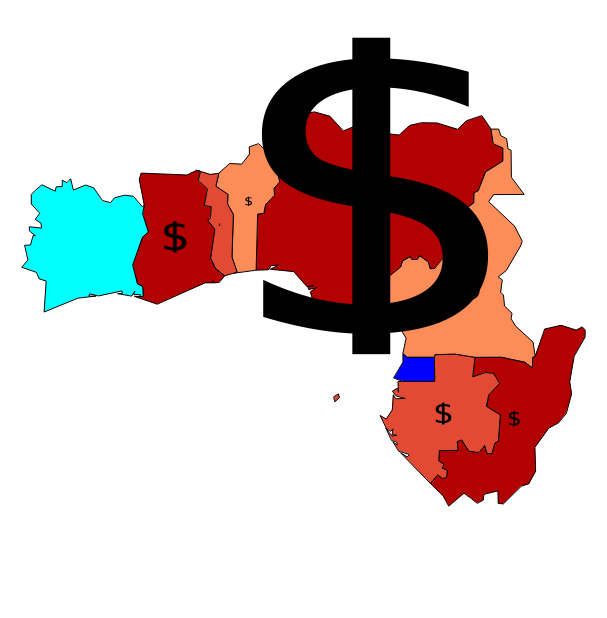
\includegraphics[width=.2\textwidth]{head.png}}
 
\usepackage{beamerthemeshadow}
%\usepackage{beamerthemesplit}
\usepackage{listings}

\newcommand{\soooo}{H$_2$SO$_4$}

%fdl stuff
\usepackage{hyperref}
\hypersetup{colorlinks, 
           citecolor=black,
           filecolor=black,
           linkcolor=black,
           urlcolor=black,
           bookmarksopen=true,
           pdftex}

\hfuzz = .6pt % avoid black boxes

\lstset{language=SQL}

\begin{document}
\setbeamertemplate{footline}[page number]
\setbeamertemplate{navigation symbols}{}
\begin{frame}
%\titlepage

\begin{titlepage}
  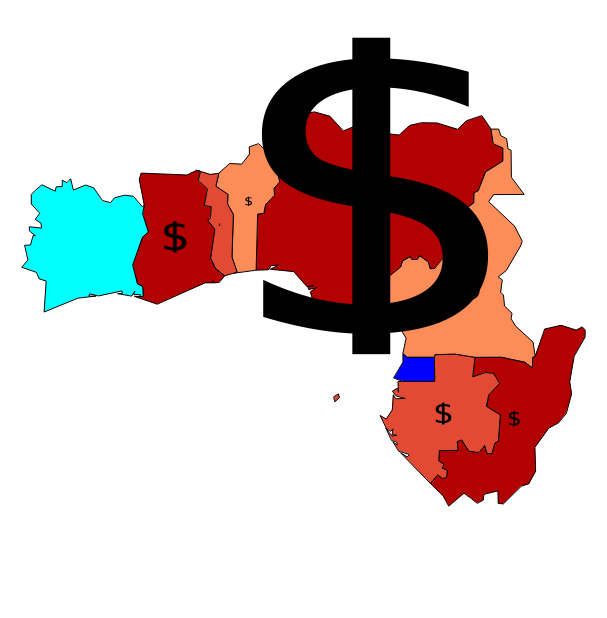
\includegraphics[height=.15\textheight]{head.png}
  %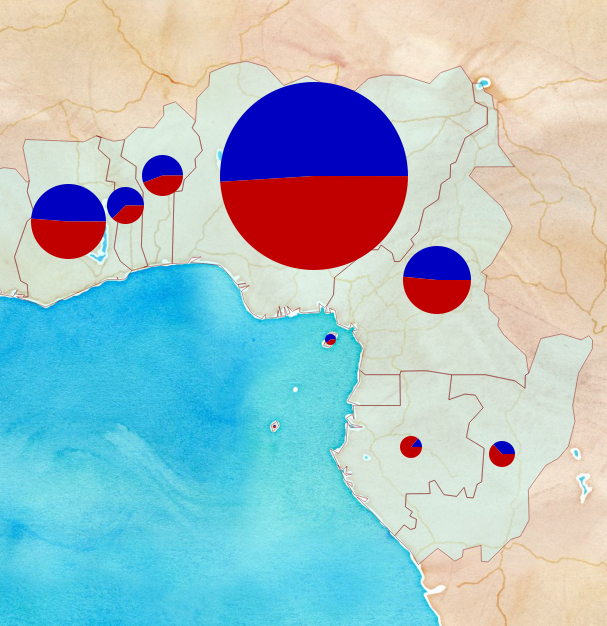
\includegraphics[height=.15\textheight]{head3.png}
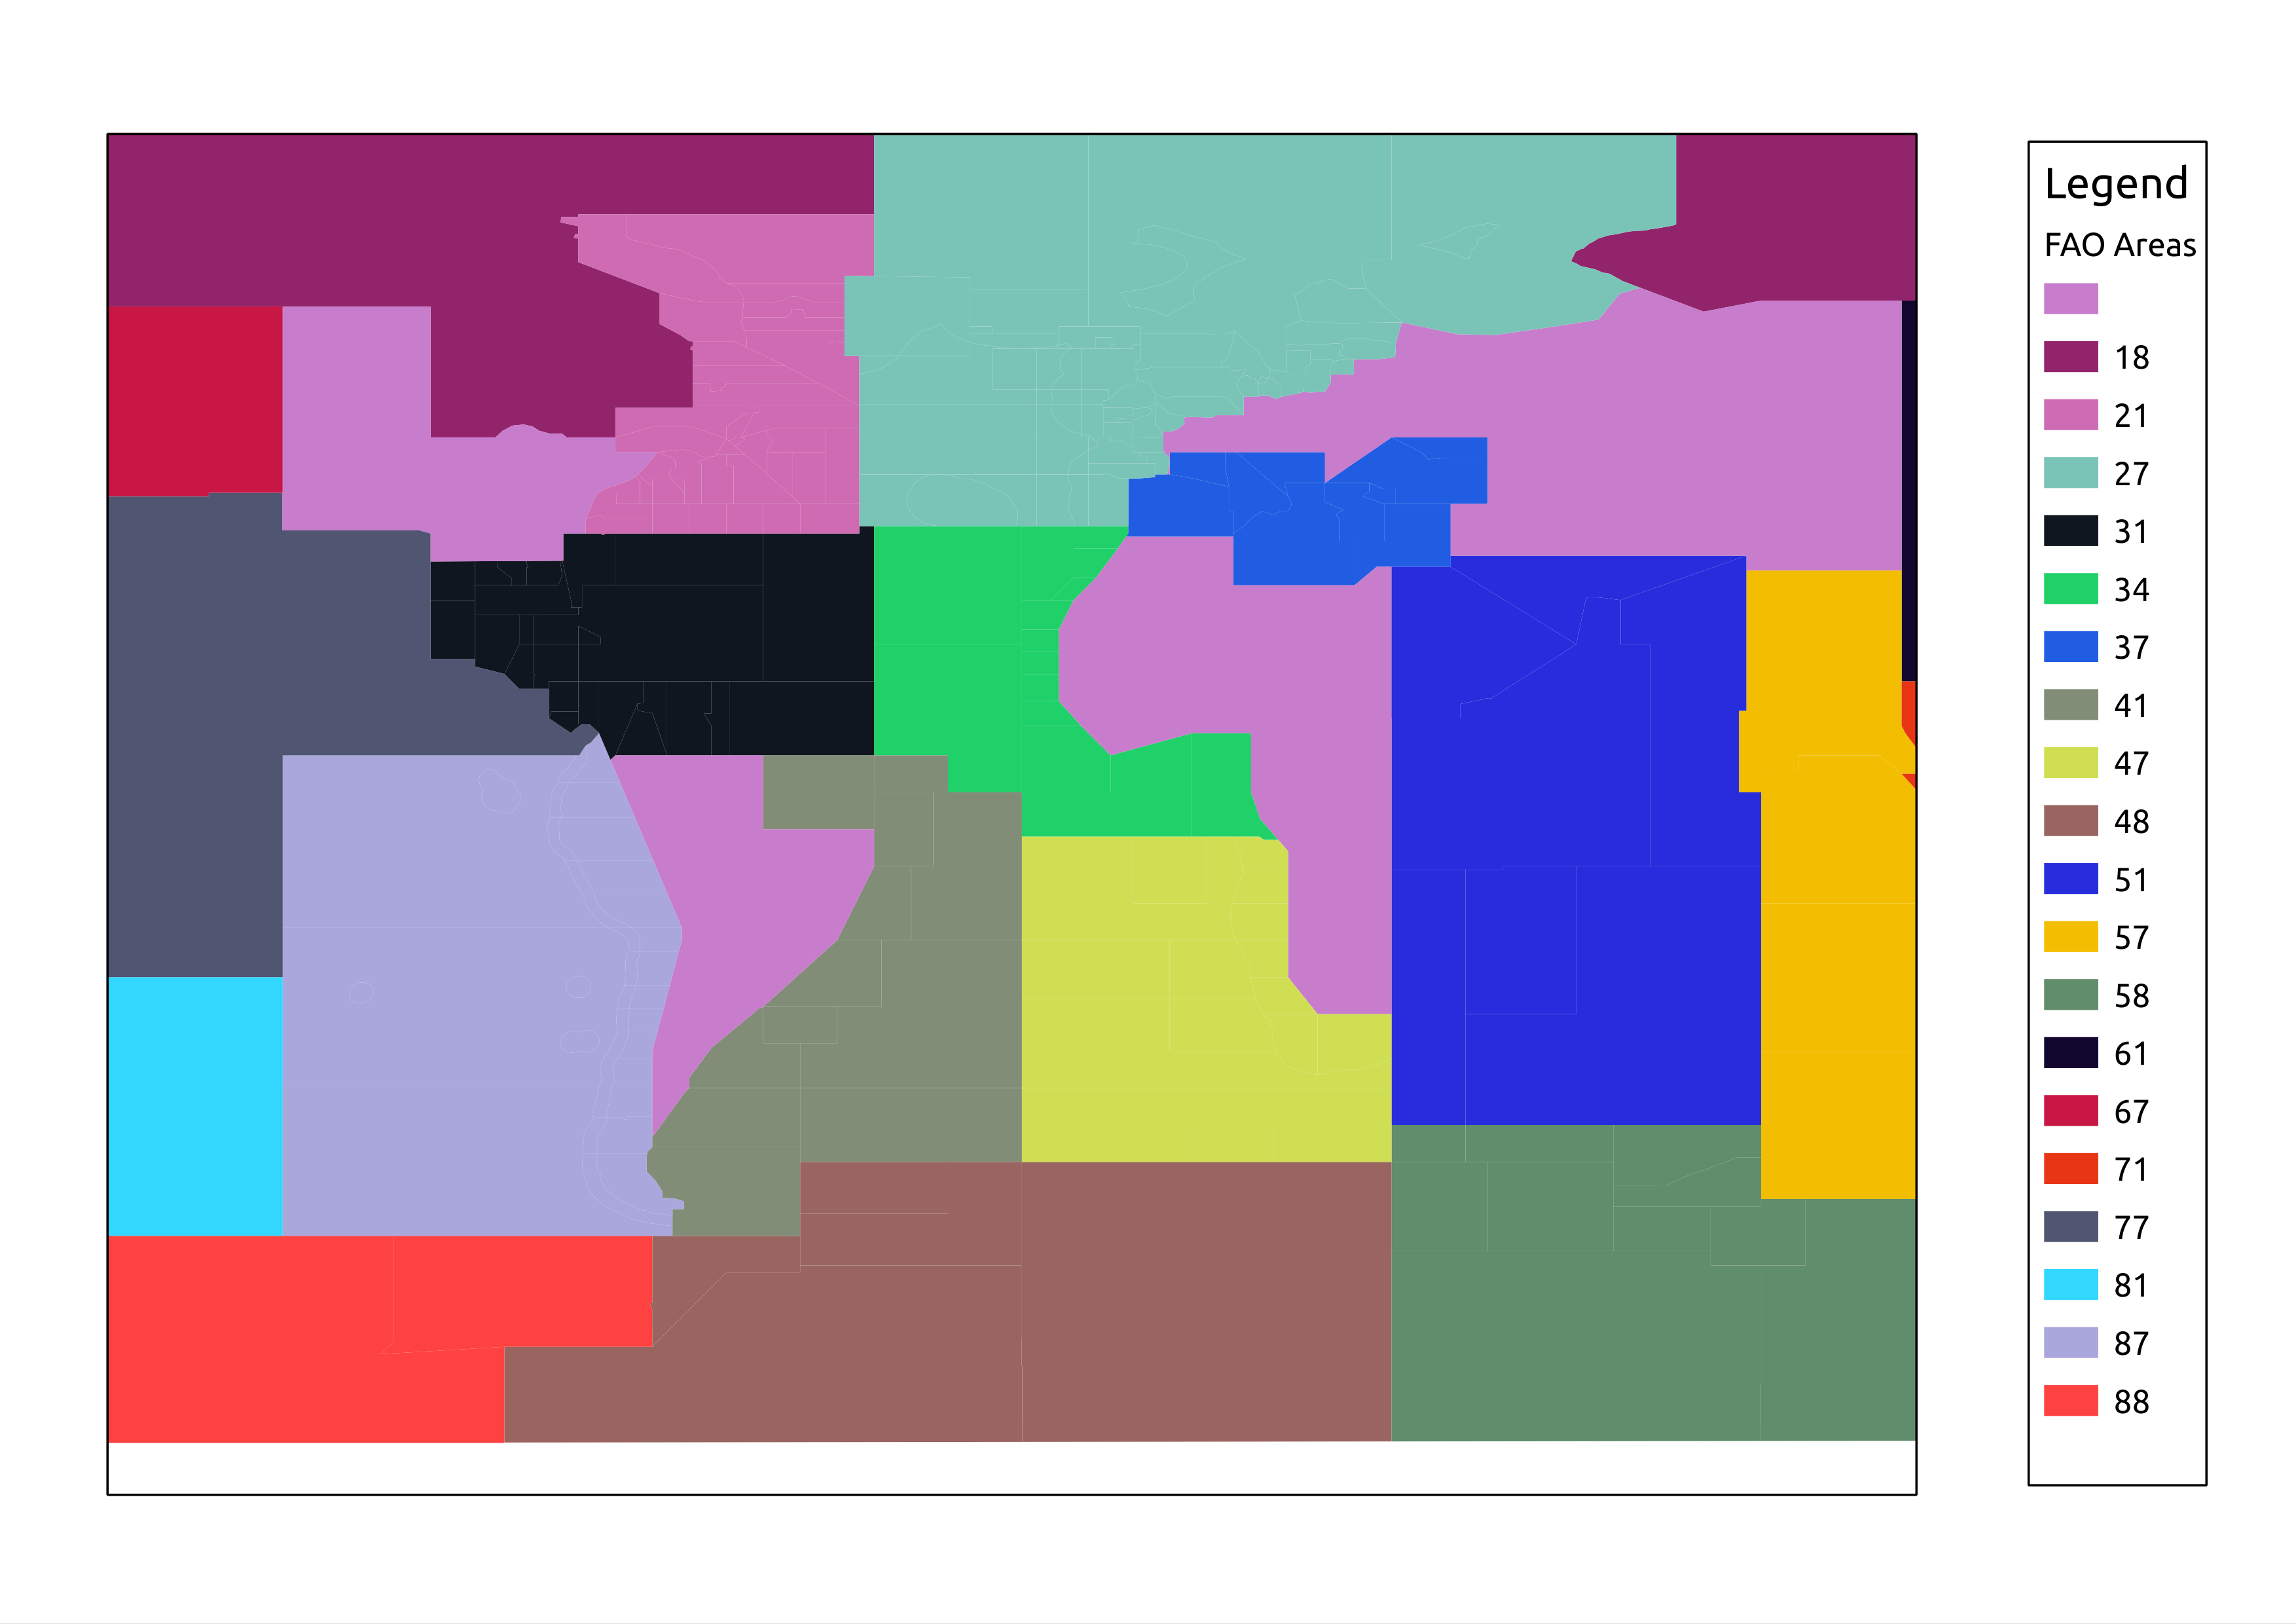
\includegraphics[height=.15\textheight]{head10.png}
  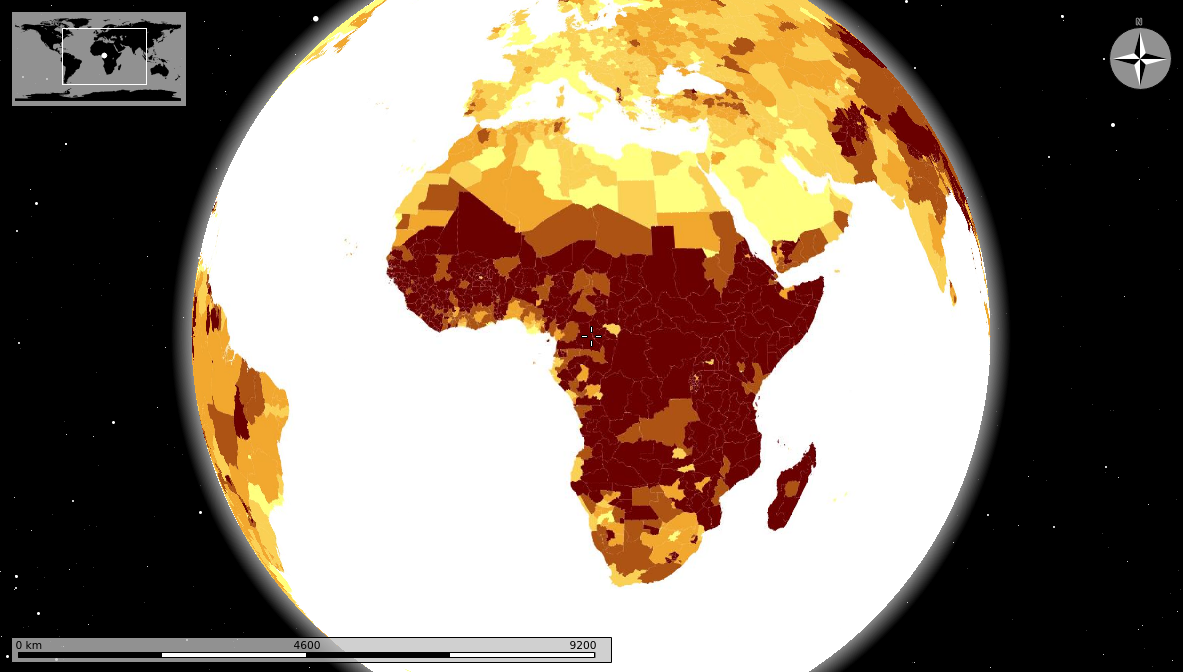
\includegraphics[height=.15\textheight]{head4.png}
  %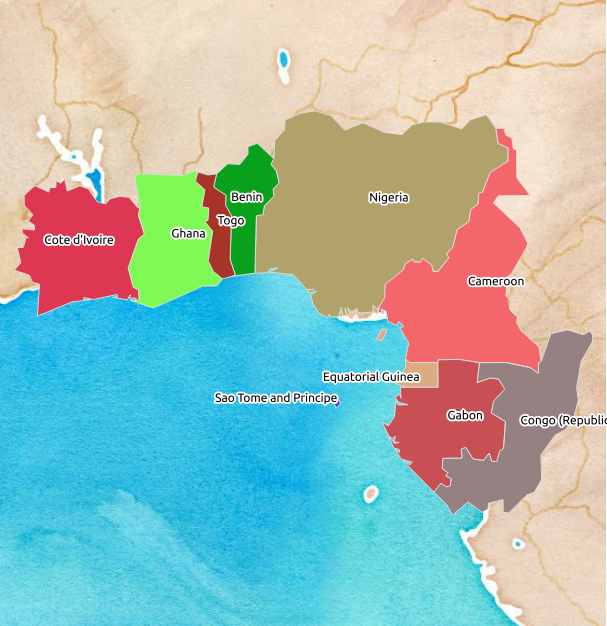
\includegraphics[height=.15\textheight]{head5.png}
  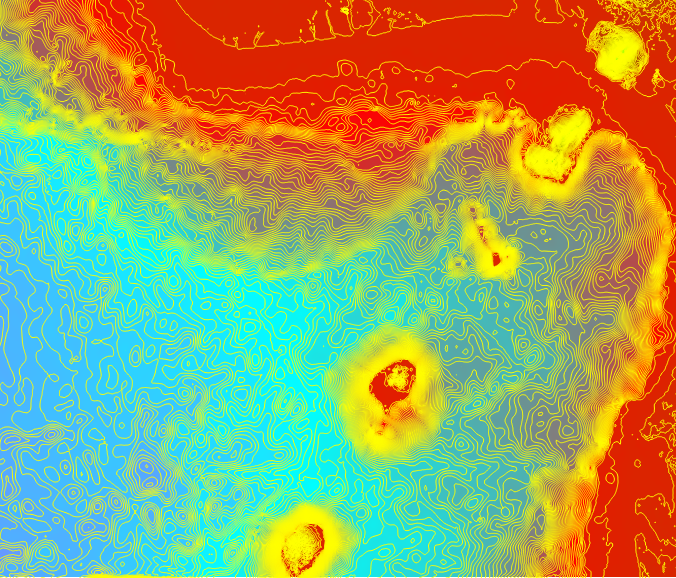
\includegraphics[height=.15\textheight]{head6.png}
%   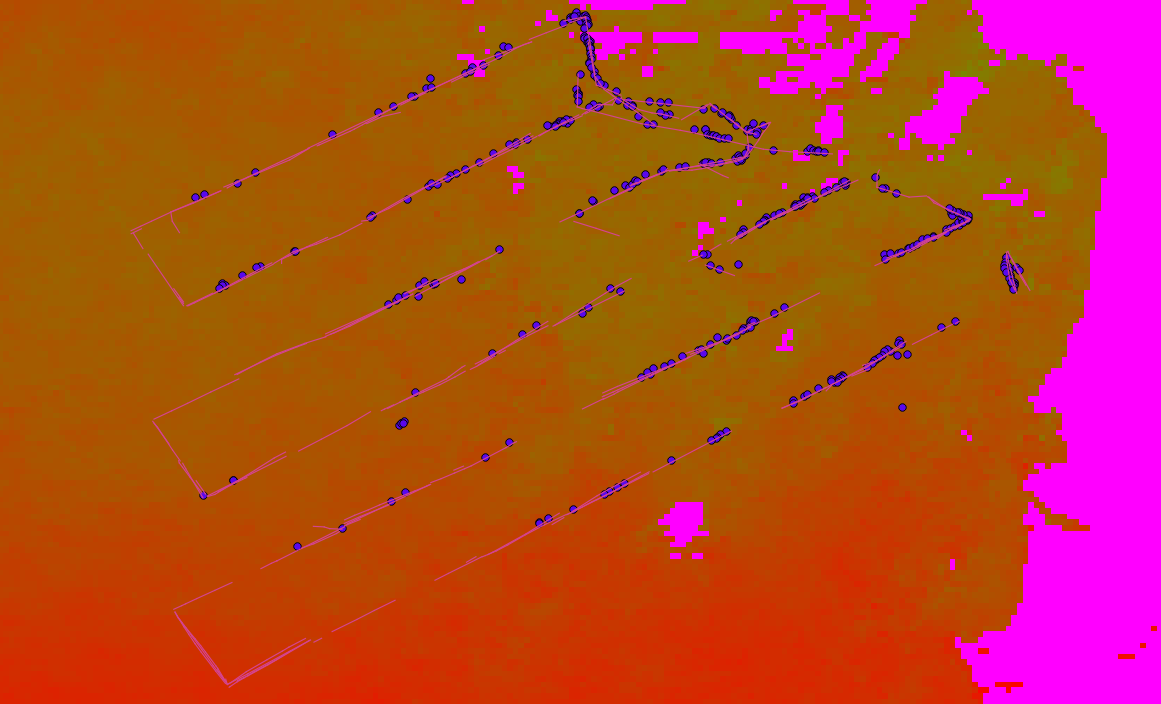
\includegraphics[height=.15\textheight]{head7.png}
  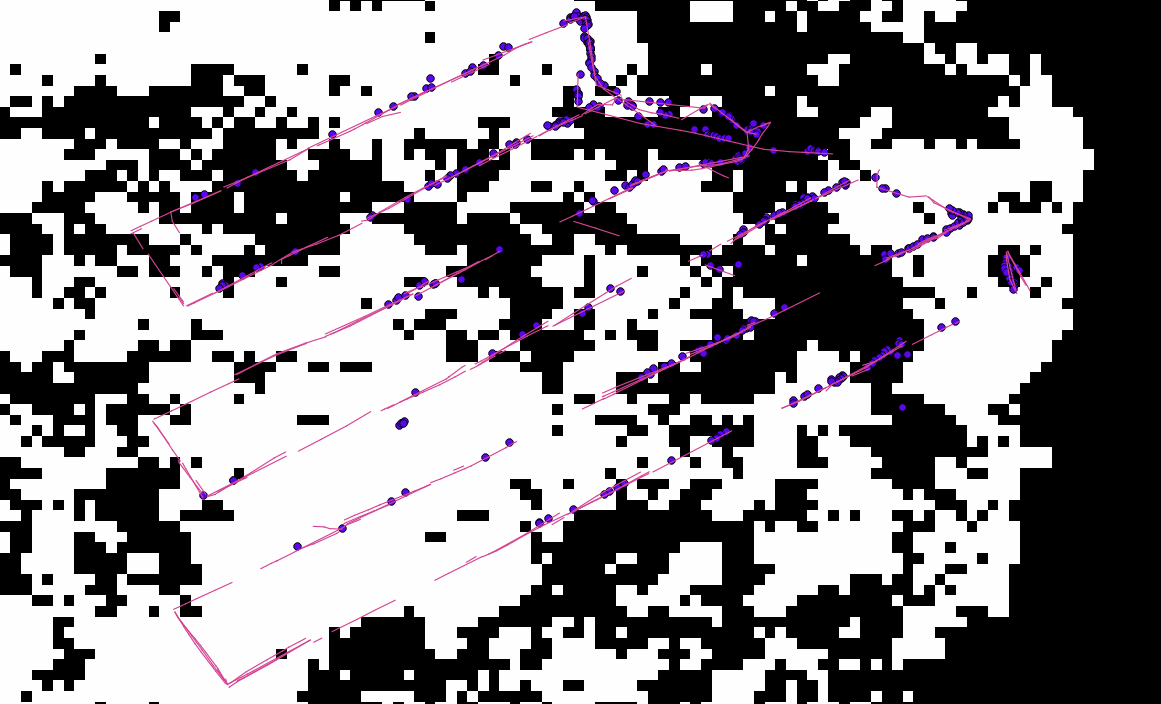
\includegraphics[height=.15\textheight]{head8.png}
  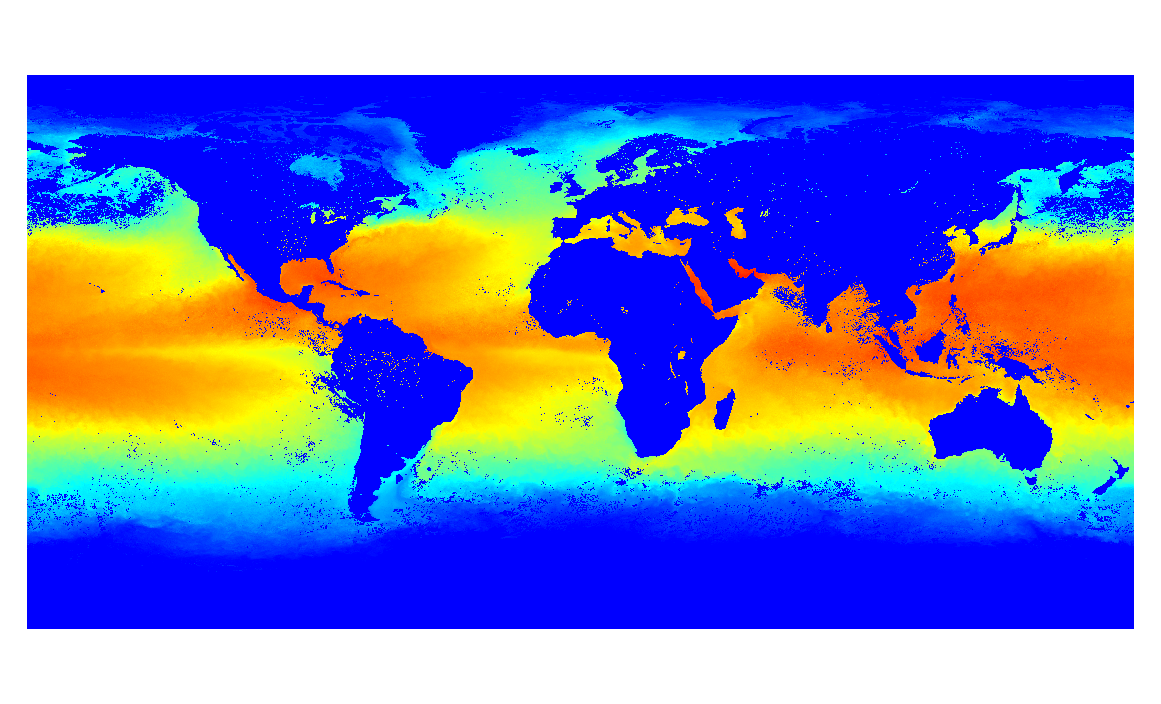
\includegraphics[height=.15\textheight]{head9.png}
  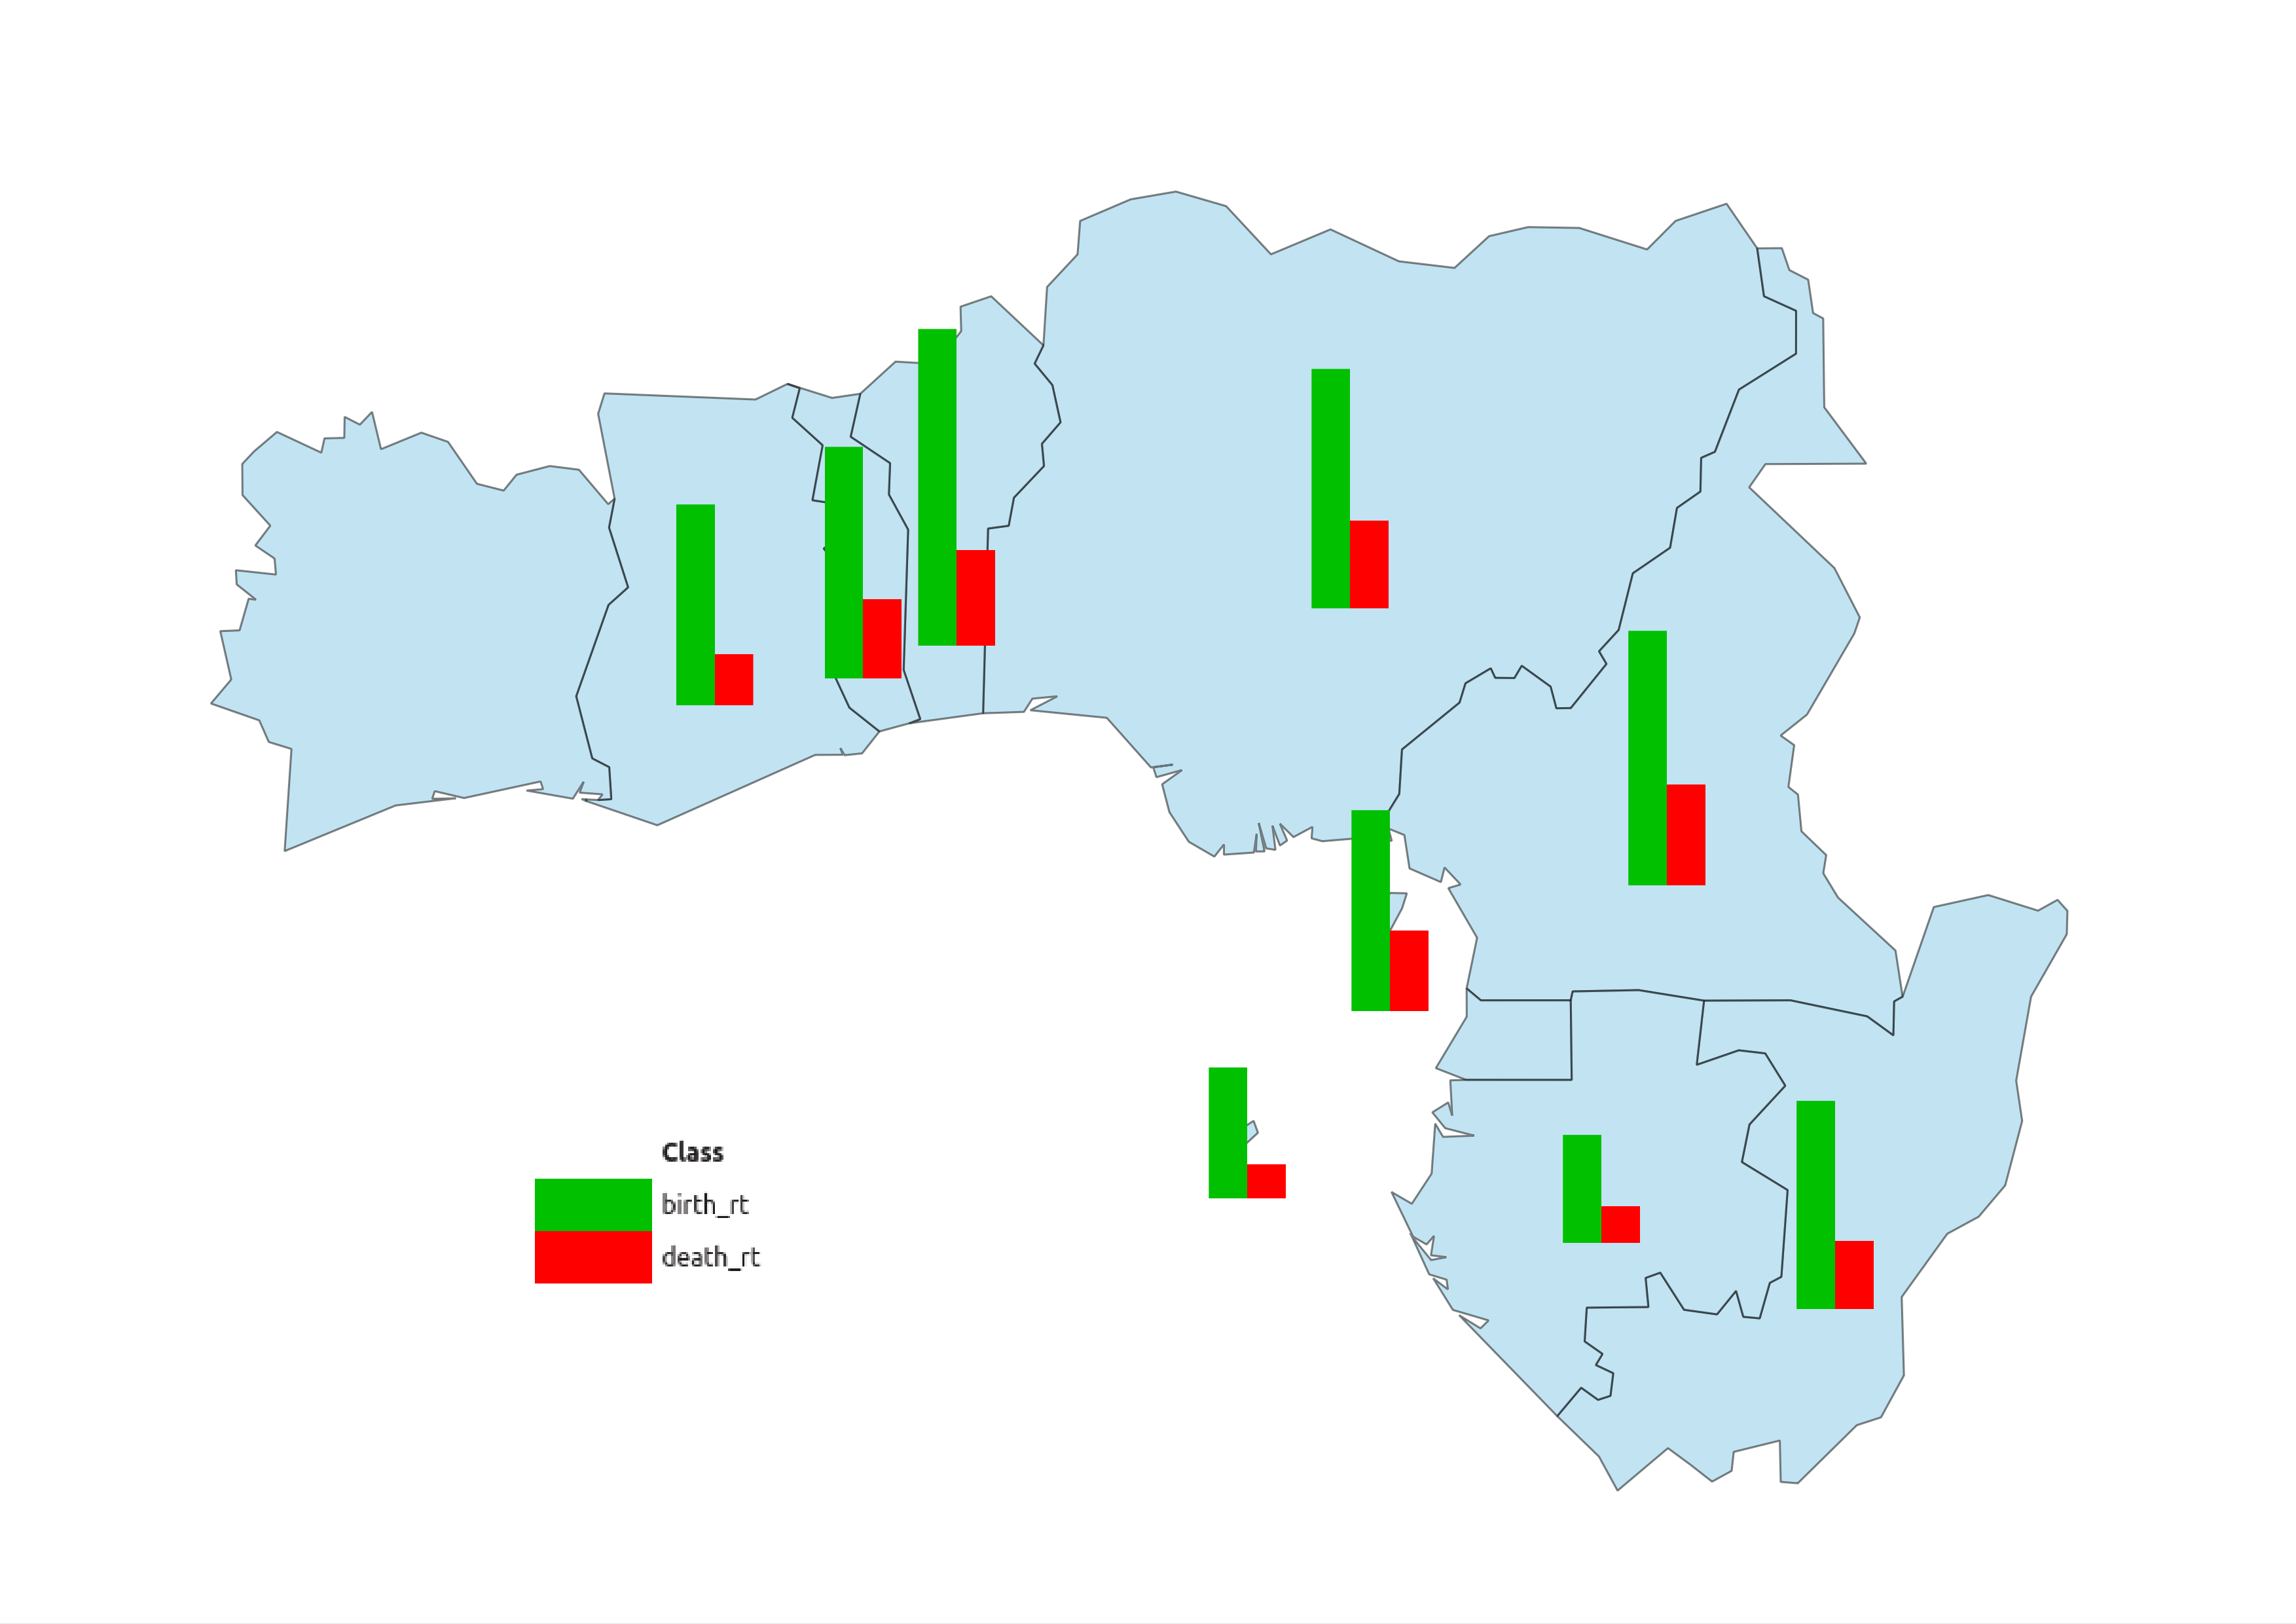
\includegraphics[height=.15\textheight]{head2.png}
\end{titlepage}

\end{frame} 
 
\begin{frame}
\frametitle{Tabela de Conte\'{u}dos}
\tiny{
\tableofcontents}
\end{frame}

\section{Introdu\c{c}\~{a}o} 
\begin{frame}
\frametitle{Introdu\c{c}\~{a}o}
Quem s\~{a}o os principais destinat\'{a}rios desta comunica\c{c}\~{a}o?
    \begin{itemize}
      \item<2-> pessoas que desenvolvem projectos de software, com tecnologias espaciais;
      \item<3-> pessoas cuja equipa onde est\~{a}o integradas n\~{a}o se dedica como actividade prim\'{a}ria \`{a} implementacao de software (ex: c\^{a}mara municipal, escola, instituto de investiga\c{c}\~{a}o aplicada, etc);
      %\item<4-> Cenario: um ou mais desenvolvedores, um ou mais \textit{stakeholders} (pessoas "interessadas" no projecto), e um \textit{use case} com uma componente espacial (ex: um sistema de aviso de cheias).
%Estas sao algumas reflexoes (nao necessariamente por ordem cronologica ou de importancia)
      \end{itemize}
\end{frame}

\section{Escolha de Ferramentas Adequadas} 
\begin{frame}
\frametitle{Escolha de Ferramentas Adequadas}

\textit{The right tool, for the right job}\\~\\

Do ponto de vista do \textit{developer}:
    \begin{itemize}
      \item<2-> n\~{a}o existem solu\c{c}\~{o}es "perfeitas"!;%as linguagens de programacao e os softwares sao motivo de discussoes "apaixonadas"; uma linguagem  de programacao nao em absoluto 'e melhor que a outra; pode depender do contexto
      \item<3-> avaliar qual \'{e} a melhor tecnologia para os objectivos que se pretendem;%DAR UM EXEMPLO COM LINGUAGEM E SOFTWARE SIG; nao 'e uma boa ideia utilizar C++ ou SQL para parse de texto, ou utilizar perl para optimizacao de memoria;
      \item<4-> ter em conta a linguagem/ferramenta em que se esta mais "confort\'{a}vel", e pesar o tempo/esfor\c{c}o em aprender uma nova;%pode ser que a linguagem mais optimizada para programar em QGIS seja C++, mas se eu sei python, nao ha problema em utilizar os bindings de python.
      \item<5-> remover os custos ligados \`{a} aquisi\c{c}\~{a}o de software propriet\'{a}rio;%financiar o desenvolvimento de uma determinada funcionalidade em FOSS (desenvolver mais)
%BUDGET/TEMPO
      \end{itemize}
\end{frame}

\begin{frame}
\frametitle{Escolha de Ferramentas Adequadas (+)}
Do ponto de vista dos recipientes:%recipientes
    \begin{itemize}
      \item<2-> normalmente os sistemas mais "simples" s\~{a}o aqueles que se aguentam mais tempo; sistemas muito sofisticados t\^{e}em invariavelmente uma manunten\c{c}\~{a}o complicada e cara!% em Africa algumas das BD que ainda estao em utilizacao foram feitas em ACCESS
      \item<3-> evitar tecnologias \textit{cutting edge}, que ainda n\~{a}o possuem uma base de conhecimento s\'{o}lida em todo o mundo; % por exemplo, o NoSQL 'e tentador, mas existem mts mais pessoas a entender e saber trabalhar com BD relacionais
      \item<4-> sempre que poss\'{i}vel, optar por standards (ex: OGC) e "fugir" de formatos e software proprietario; os standards em princ\'{i}pio garantem uma continuidade no tempo e no espa\c{c}o;% um exemplo comum, sao formatos de ficheiros nao documentados, que contem uma quantidade valiosa de dados, mas os programadores foram-se embora, e levaram com eles a especificacao na sua cabeca; com o software proprietario tambem estamos sempre nao mao da empresa, que pode por exemplo decidir descontinua-lo e remover apoio a versoes anteriores (por isso optar por FOSS)
      \item<5-> pensar tamb\'{e}m nas restri\c{c}\~{o}es de \textit{hardware} dos recipientes: t\^{e}em acesso \`{a} internet?  t\^{e}em multi core, que resolu\c{c}\~{a}o t\^{e}em?% o acesso a internet 'e particularmente importante na area dos Geo webservices; 'e comum planear o sistema numa BD centralizada, com clientes distribuidos para visualizar e introduzir dados (Ex: Mapserver, GeoServer + MySQL ou PostGres); No entanto, se os utilizadores trabalham offline (porque por exemplo estao num barco), fica o sistema inutilizavel;
      \end{itemize}
\end{frame}

\section{FOSS} 
\begin{frame}
\frametitle{Software Livre e de C\'{o}digo Aberto}
  %Definicao: software que respeita as quatro liberdades fundamentais (por link aqui)
    
\includegraphics[scale=0.2]{gnu.png}
    \tiny{\url{http://www.gnu.org/philosophy/free-sw.html}}\\~\\
\small{
Para al\'{e}m do custo "zero" e das motiva\c{c}\~{o}es "\'{e}ticas":
    \begin{itemize}
      \item<2-> \textbf{custos de \textit{hardware} mais baixos:} geralmente o software FOSS requer menos capacidade computacional para realizar as mesmas tarefas que em servidores "convencionais" ou \textit{workstations}.%E.g.Windows, solaris. Isto permite instala-lo em hardware antigo, em clientes com menos recursos.
      \item<3-> \textbf{gest\~{a}o de licen\c{c}as simplificada:} podem obter-se quantas licen\c{c}as se quiser, para instalar em toda a parte, o que quer dizer que a produtividade n\~{a}o \'{e} afectada por quest\~{o}es de licen\c{c}as. %por exemplo, em software proprietario pode acontecer haver apenas um computador com a licenca (hardware key), e as pessoas teem de esperar para utiliza lo;
      \end{itemize}
}
\end{frame}

\begin{frame}
\frametitle{Software Livre e de C\'{o}digo Aberto (+)}
\small{
    \begin{itemize}
      \item<1-> \textbf{amplo suporte:} o suporte para FOSS \'{e} muitas vezes superior ao de solu\c{c}\~{o}es propriet \'{a}rias. Isto deve-se s que existem dois n \'{i}veis de suporte: o gratuito, providenciado pela comunidade online (em crescimento) e o pago, que muitas companhias agora disponibilizam (ex: Novell).%em relacao ao gratuito, posso dizer que recentemente lidei com um bug na versao do Windows do QGIS/Sextante, e ao por os meus problemas na mailing list, obtive respostas, muitas vezes em questao de minutos; a interaccao foi quase em "tempo real";
      \item<2-> \textbf{qualidade de software:} o processo de revis\~{a}o pelos pares e os standards da comunidade, adicionados ao facto de que o c\'{o}digo \'{e} revelado a todos, tendem a promover a "excel\^{e}ncia" em \textit{design} e \textit{coding};
      \item<3-> \textbf{"vida" extendida:} a disponibilidade do c\'{o}digo fonte e o direito de o modificar ("liberdade" numero 1) possibilita o melhoramento ilimitado do software. Tambem possiblita port\'{a}-lo para um novo \textit{hardware} ou sistema operativo. O direito de distribuir as vers\~{o}es modificadas ("liberdade" 3) possibilita as actualiza\c{c}\~{o}es frequentes.
%Na realidade aplicacoes apenas binarias nao costumam sobreviver mais do que 10 anos na forma nao-modificada, enquanto sistemas abertos sobreviveram mais de 30 anos (DAR EXEMPLO)
      \end{itemize}
}
\end{frame}

%\begin{frame}
%\frametitle{Software Livre e de Codigo Aberto (+)}
%\small{
%    \begin{itemize}
%      \item<1-> actualizacoes frequentes: nao e necessario ser um programador para beneficiar da disponibilidade de estudar codigo fonte ("liberdade" 1); esta liberdade atrai uma comunidade de desenvolvedores,  que corrige bugs e desenvolve novas funcionalidades; o direito de distribuir as versoes modificadas ("liberdade" 3) permite a comunidade de utilizadores beneficiar de todos estes melhoramentos.
%      \item<2-> comunidade em crescimento: o direito de utilizar o software de qualquer forma, combinado com direitos de redistribuicao, atrai uma grande base de utilizadores, que ajuda a construir um mercado de suporte e costumizacao, que por sua vez atrai ainda mais desenvolvedores a trabalhar no projecto. %Se o software e util, existe feedback que guia a qualidade do produto, melhor a sua funcionalidade e suporte;
%      \end{itemize}
%}
%\end{frame}

\begin{frame}
\frametitle{Software Livre e de C\'{o}digo Aberto (+)}

\textit{Milestone} na historia do FOSS em Portugal:
\\~\\
\pause
Recentemente o Tribunal anulou um concurso p\'{u}blico relativo ao licenciamento e manunten\c{c}\~{a}o de software Microsoft, lan\c{c}ado por uma c\^{a}mara municipal.
%As sepcificacoes tecnicas do concurso impediam que qualquer empresa que nao a microsoft (ou partners) concorressem.
%considerou se que isto desrespeita as regras de contratacao publica (fomentar a livre concorrerncia), e espera-se que o ganhar desta cause venha quebrar um padrao nas empresas publicas, por mts anos.

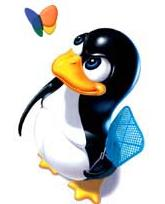
\includegraphics[scale=0.5]{windows2.jpg}

\small{Ler a hist\'{o}ria completa:
\url{http://tinyurl.com/bx42shh}
}
\end{frame}

\section{Informa\c{c}\~{a}o Espacial}
\begin{frame}
\frametitle{Identificar a Informa\c{c}\~{a}o Espacial}

A informa\c{c}\~{a}o espacial pode j\'{a} estar inclu\'{i}da nos dados, embora os \textit{stakeholders} n\~{a}o estejam cientes disso.
H\'{a} que identific\'{a}-la e represent\'{a}-la de forma adequada.


\includegraphics[scale=0.3]{detective.png}
\end{frame}


\begin{frame}
\frametitle{Exemplo: Pontos como Coordenadas}

%TODO: write something here

\begin{columns}
  \begin{column}{5cm}
    \begin{figure}
    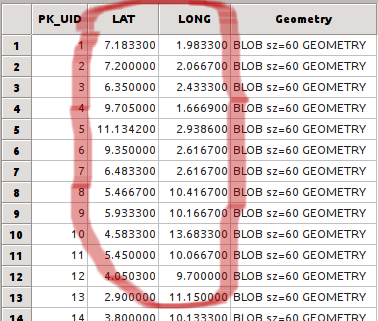
\includegraphics[scale=0.4]{geometry3.png}
    \end{figure}
  \end{column}
  \begin{column}{5cm}
    \begin{figure}
    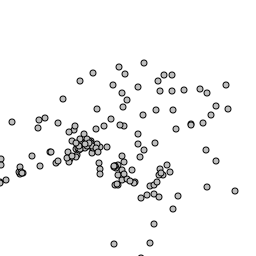
\includegraphics[scale=0.33]{geometry.png}
    \end{figure}
  \end{column}  
\end{columns}

\end{frame}

\begin{frame}
\frametitle{Exemplo: Pontos como Coordenadas (+)}

%TODO: write something here

\tiny{
\begin{tabular}{ l l }
  WKT: & POINT(1.9833 7.1833) \\
  EWKT: & $SRID=4326;POINT(1.9832999706 7.1833000183)$ \\
  SVG: &  x="1.9833" y="-7.1833" \\
  KML: & $<Point><coordinates>1.9832999706,7.1833000183</coordinates></Point>$ \\
  GeoJSON: & ${"type":"Point","coordinates":[1.9832999706,7.1833000183]}$ \\
\end{tabular}
}

\end{frame}
 
\begin{frame}
\frametitle{Exemplo: Pol\'{i}gonos como Atributos Nominais}

%As fishing zones (ou zonas de pesca) sao apresentadas como uma lista de nomes, numa tabela de referencia (a qual se ligam outras tabelas por chaves estrangeiras); na realidade, estas "zonas" sao na realidade poligonos, como podemos ver no servidor WMS da FAO;

\begin{columns}
  \begin{column}{0.5\textwidth}
    \begin{figure}
    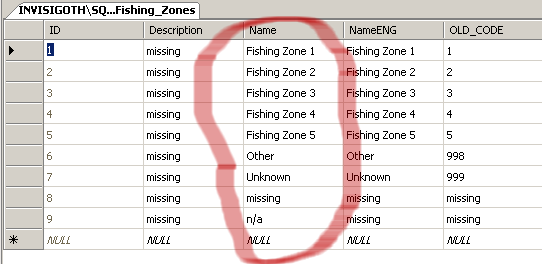
\includegraphics[scale=0.22]{fishing_zones1.png}
    \end{figure}
  \end{column}
  \begin{column}{0.5\textwidth}
    \begin{figure}
    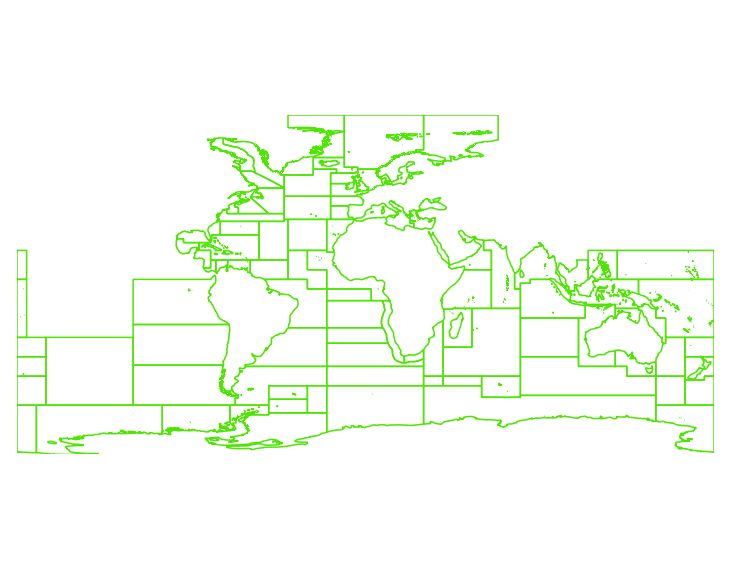
\includegraphics[scale=0.22]{fishing_zones2.png}
    \end{figure}
\tiny{
\url{http://data.fao.org/maps/ows?SERVICE=WMS&REQUEST=GetMap&layers=GEONETWORK:fa_subareas_31627&width=800&height=600&FORMAT=image/png&CRS=EPSG:4326&BBOX=-180,-90,180,90}
}
  \end{column}  
\end{columns}

\end{frame}

\begin{frame}
\frametitle{Representar a Informa\c{c}\~{a}o Espacial}

Em \'{u}ltima inst\^{a}ncia a forma como representamos os dados espaciais, vai determinar as opera\c{c}\~{o}es que podemos fazer com eles.

\end{frame}

\begin{frame}
\frametitle{Representar as Informa\c{c}\~{a}o Espacial (+)}

Uma "esta\c{c}\~{a}o" de arrasto (recolha de amostras de pesca), pode ser armazenada como:

\begin{columns}
  \begin{column}{0.5\textwidth}

    \begin{itemize}
      \item<2-> uma sequ\^{e}ncia de pontos;
      \item<3-> uma linha;%unindo todos os pontos
      \item<4-> um pol\'{i}gono.%incluindo a largura da rede de arrasto
      \end{itemize}


  \end{column}
  \begin{column}{0.5\textwidth}
    \begin{figure}
      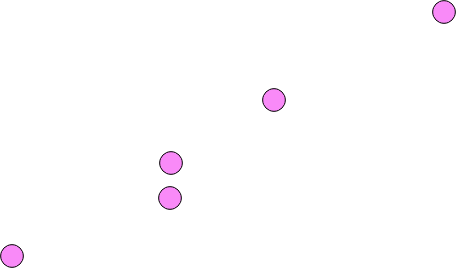
\includegraphics[width=0.3\textwidth]{trawl_pts.png}
    \end{figure}
    \begin{figure}
      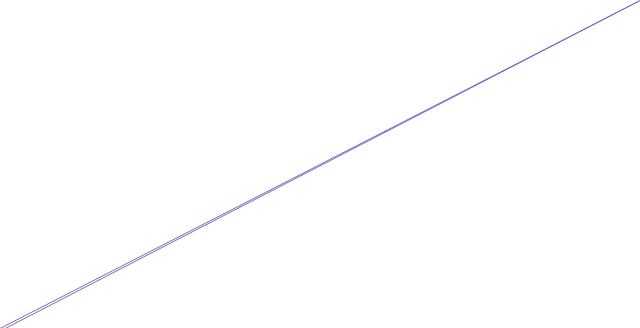
\includegraphics[width=0.3\textwidth]{trawl_lines.png}
    \end{figure}
    \begin{figure}
      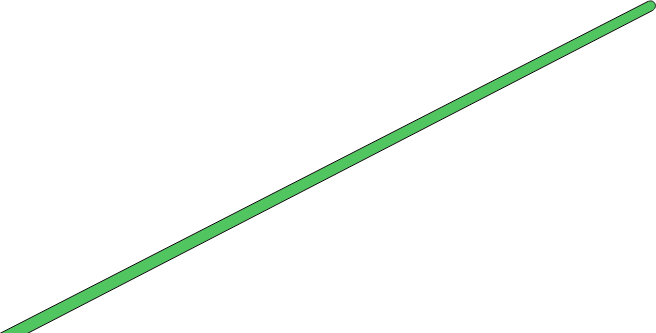
\includegraphics[width=0.3\textwidth]{trawl_poly.png}
    \end{figure}
  \end{column}  
\end{columns}
\end{frame}

\begin{frame}[fragile]
\frametitle{Representar a Informa\c{c}\~{a}o Espacial (+)}

Se queremos calcular a \'{a}rea arrastada, qual \'{e} a representa\c{c}\~{a}o mais adequada?
\\~\\

\tiny{
\pause
\begin{lstlisting}
pts: select area( buffer(Makeline(geometry), 0.5) ) from trawl_points a order by rowid
\end{lstlisting}
\pause
\begin{lstlisting}
linha: select area( buffer(a.geometry, 0.5)  ) from trawl_lines as a
\end{lstlisting}
\pause
\begin{lstlisting}
poligono select area(geometry) from trawl_polygons
\end{lstlisting}


%area=201472.064690 m

}
\end{frame}

%\begin{frame}
%\frametitle{Fontes de Dados}
%\begin{overprint}

%sempre o problema dos dados
%dados gratuitos: existem mts dados - avaliar a possibilidade de os integrar
%hj em dia existem fontes mais "informais" de dados (redes sociais)

%\end{overprint}
%\end{frame}

\section{AGILE}
\begin{frame}
\frametitle{AGILE}
Agile \'{e} um conjunto de pr\'{a}ticas de desenvolvimento de software, de forma \textbf{iterativa} e \textbf{incremental}, 
resumido nos 12 princ\'{i}pios do manifesto (2001):

\centering{ \tiny{
\url{http://www.agilemanifesto.org/principles.html}
} }

\begin{itemize}
  \item<2-> favorecer indiv\'{i}duos e interac\c{c}\~{o}es, em detrimento de processos e ferramentas;
  \item<3-> favorecer software que funciona, em detrimento de extensa documenta\c{c}\~{a}o;%favorecer o desenvolvimento em relacao as especificacoes; 
  \item<4-> favorecer colabora\c{c}\~{a}o dos \textit{stakeholders}, em detrimento de negocia\c{c}\~{a}o de contratos;%privilegiar em a comunicacao a todos os niveis, entre os elementos ("partilhar" os sucessos e os fracassos);
  \item<5-> favorecer resposta \`{a} mudan\c{c}a, em detrimento de "seguir um plano";% flexibilidade de requerimentos
\end{itemize}

%surgiu como reaccao ao waterfall model: ao entregar software funcional, testado e pronto a distribuir numa base incremental, Agile entrega valor
 %acrescentado, visibilidade e adaptabilidade, muito mais cedo no ciclo de desenvolvimento de software, reduzindo significativamente os riscos
%do projecto

\end{frame}

\begin{frame}
\frametitle{AGILE (+)}
O desenvolvimento AGILE est\'{a} francamente estabelecido na ind\'{u}stria de software, mas n\~{a}o suficientemente na \'{a}rea dos SIG. %menos bugs, e resultados mais rapidos

%Survey: \url{http://tinyurl.com/p4gdhps}

    \begin{figure}
      
\includegraphics[width=0.3\textwidth]{agile1.jpg}
    \end{figure}

\small{
Numa survey realizada em 2008, apenas 23\% dos \textit{developers} de SIG utilizavam pr\'{a}ticas AGILE (contra 69\% dos \textit{developers} de software \textit{mainstream}).\\
\tiny{
survey: \url{http://edgehopper.com/results-of-agile-gis-survey/}
}
}
\end{frame}

\begin{frame}
\frametitle{Mitos}

Alguns "mitos" sobre a implementa\c{c}\~{a}o de metodologias Agile: %ou ideias erradas
\begin{itemize}
  %\item<2-> nao se aplica a projectos de SIG;%agile aplica se a qualquer projecto de desenvolvimento de software (e nao so), por isso aplica se ao caso de utilizar tecnologias espaciais.
  \item<2-> s\'{o} se aplica em equipas de desenvolvimento de software com v\'{a}rias pessoas, ou em projectos de grande dimens\~{a}o;% embora haja um numero optimo de elementos na equipa AGILE, ele pode ser reduzido ao minimo (caso em que uma ou mais pessoas acumulam roles)
  \item<3-> \'{e} obrigat\'{o}rio implementar todas as pr\'{a}ticas Agile;%: pode usar se uma ou muitas coisas do agile. 
  \item<4-> toma muito tempo;%agile evita os "atrasos" e reduz os bugs, por isso pode dizer-se que 'e o oposto de tomar tempo
\end{itemize}

\end{frame}

%\begin{frame}
%\frametitle{Metodologias}
%Exemplos: Scrum, TTD, XP; \\~\\%vale a pena ler um pouco mais sobre elas

%Da minha experiencia em projectos, retenho os seguintes "conceitos" Agile:
%\begin{itemize}
%  \item<2-> favorecer o desenvolvimento em relacao as especificacoes; % por a mao na massa, o mais depressa possivel
%  \item<3-> proceder iteracoes (ciclos); %ir do mais simples ao mais complexo
%  \item<4-> privilegiar em a comunicacao a todos os niveis, entre os elementos ("partilhar" os sucessos e os fracassos);%a equipa pode inclusivamente estar fisicamente separada, desde que se utilizem as ferramentas de comunicacao adequadas, (skype, wiki, etc);
%  \item<5-> flexibilidade de requerimentos; % adaptabilidade; a vantagem do agile e que ve a a mudanca como uma coisa boa, e nao uma ameaca
%  \item<6-> a tecnologia deve ser escolhida pelas pessoas que a vao implementar; % evitar hierarquias pouco produtivas, e responsabilizar cada elemento da equipa pelo seu role;
%  \item<7-> automacao; % aproveitar ao maximo os mecanismos automaticos: automatic builds, batch tests, documentacao automaticamente gerada, etc; podem levar tempo a implementar ao inicio, mas depois reduzem o tempo da release, ao longo d todo o processo;
%  \item<8-> nao descurar as caracteristicas nao funcionais do software; % obriga a constante refactoring, mas facilita a code ownership, debugging, desenvolvimento de novas features, etc; code reviews sao uma pratica boa para isto;
%\end{itemize}
%\end{frame}

\begin{frame}
\frametitle{Ferramentas Agile}
Algumas Ferramentas Agile:
\begin{itemize}
  \item comunica\c{c}\~{a}o simples, falada ou escrita (VoIP, email);%skype
  \item \textit{web-based collaborative editors} (wiki, etherpad);%piratenpad, mediawiki
  \item \textit{versioning systems} (git, Subversion, etc);
  \item ferramentas integradas de gest\~{a}o de projectos (Redmine, Trac, etc);
\end{itemize}
\end{frame}

\begin{frame}
\frametitle{Ferramentas Agile (+)}
Esta \'{e} a "melhor" ferramenta Agile:
\begin{figure}
  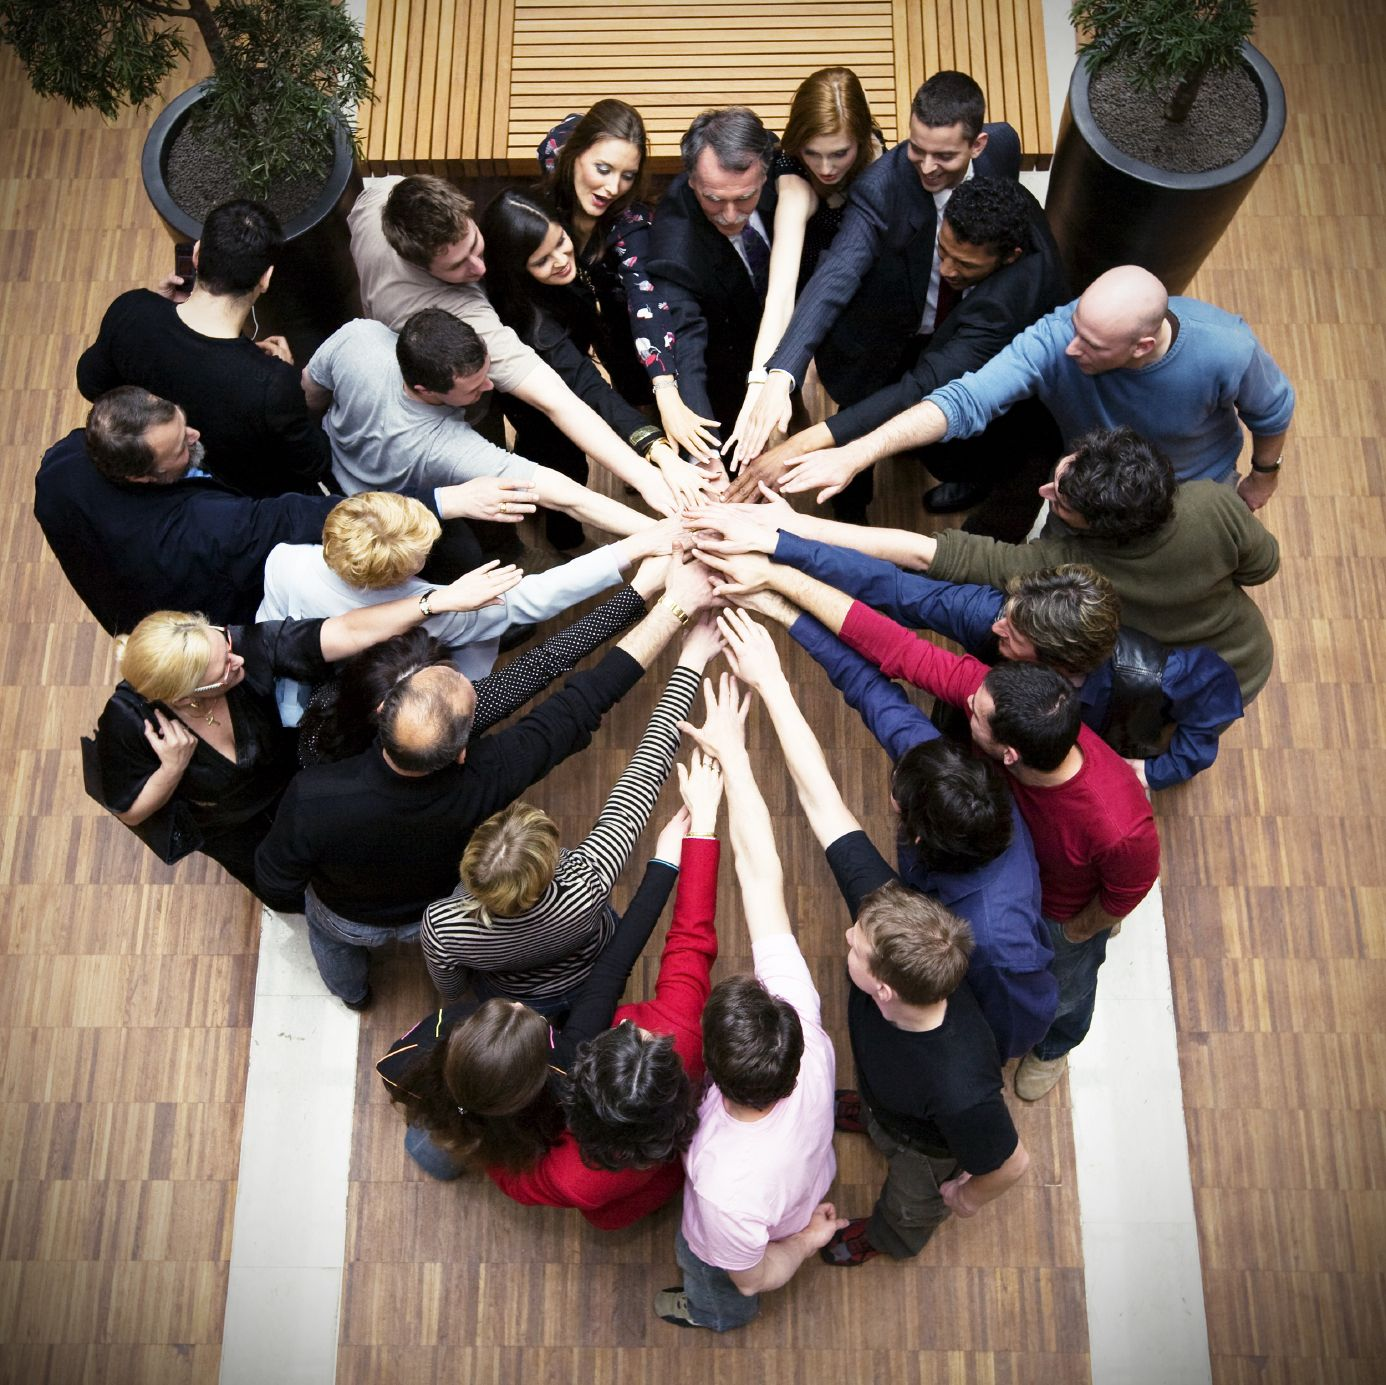
\includegraphics[width=0.5\textwidth]{agile_team.jpg}
\end{figure}
\end{frame}

\section{Sumario}
\begin{frame}
\frametitle{\textit{Roadmap} para o "sucesso":}
(Alguns) aspectos a ter em conta:
\begin{figure}
  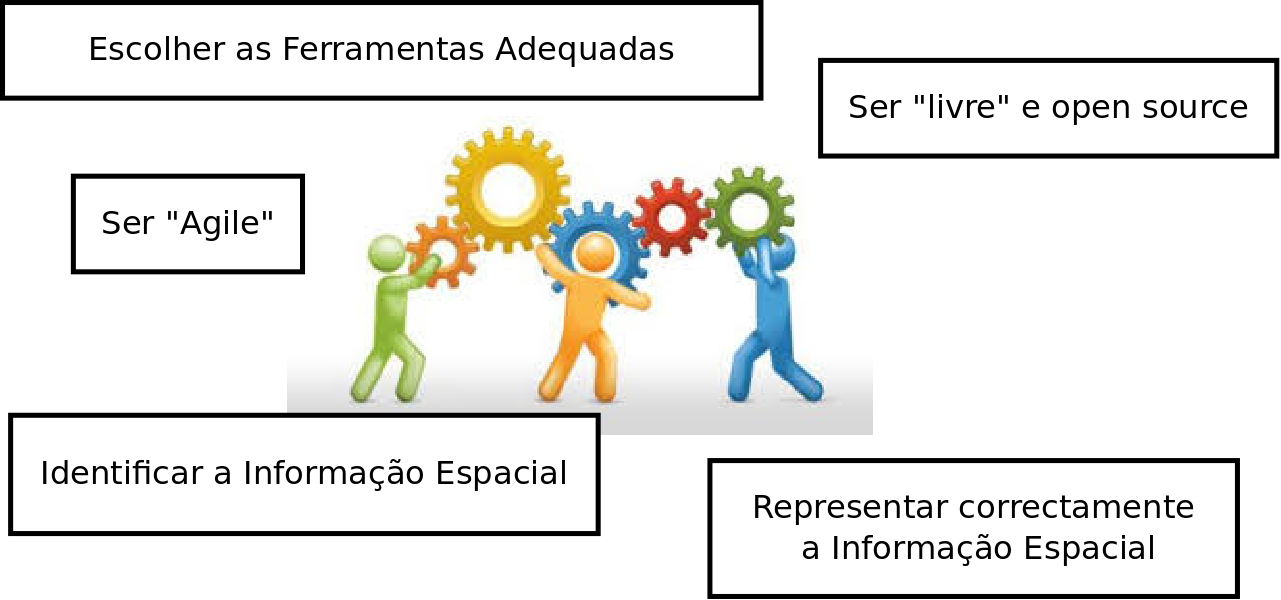
\includegraphics[width=0.7\textwidth]{Diagram1.png}
\end{figure}
\end{frame}

\section{Refer\^{e}ncias}
\begin{frame}
\frametitle{Refer\^{e}ncias}
\small{
\begin{itemize}
\item Shore, J. "The Art of Agile Development". O'Reilly Media; 1 edition (November 2, 2007)
\item Simoes, J. "Some Thoughts on Writing a Scientific Application". CVU, Vol. 4, Issue 2 (May, 2012). url: \url{http://accu.org/var/uploads/journals/cvu242.pdf}
\item Stallman, R. "Free Software, Free Society". FSF (2002). url: \url{http://www.gnu.org/doc/fsfs-ii-2.pdf}
\item \url{http://www.casa.ucl.ac.uk/joanamargarida/}
\item \url{http://www.doublebyte.net}
\end{itemize}
}
\begin{figure}
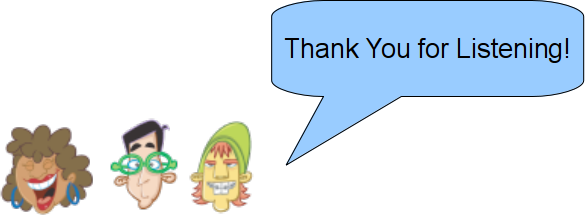
\includegraphics[scale=0.3]{thanks.png}
\end{figure}
\end{frame}


\end{document}


% 
% 
% 
% 5 - cuidar as caracteristicas nao "funcionais do projecto"; nao criar atalhos que podem ser custosos:
% 
% - tentar ir para alem da tecnologia e entender o conteudo
% 
% 
% 
% 
% 
% 
% 
% 
% 
% 
% 
% 1
% Apresentacao, etc.
% Vou basear esta apresentacao num trabalho de investigacao que desenvolvi no ultimo ano sobre ferramentas livres open-source para suportar o desenvolvimento de um plano de gestao de pescas.
% 
% 2.
% Porque utilizar FOSS?
% 
% Explicar o que 'e software FOSS e quais sao as vantagens de utilizar lo.
% 
% 
% 3.
% A quem podem interessar estas ferramentas?
% "Geohacker" pode incluir desde o utilizador mais simples, ao dba ou programador. Pode ser um cientista, um gestor, etc.
% E uma pessoa que trabalha com dados geograficos. Desta forma, penso que se aplica a cada um dos presentes no Geocamp
% 
% 4.
% Alguns nomes mais mediaticos:
% 
% QGIS, spatialite, Grass, OpenLayers, Geoserver
% 
% Em vez destes escolhi um conjunto de 3 ferramentas menos "conhecidas": 
% - um cliente de webmapping
% - uma BD raster
% - uma plataforma de modelacao
% 
% 2
% 1 Marble
% 2
% 2 librasterlite
% 2
% 3 sextante
% 
% links, etc
% 
% //////////////////// Desenvolvimento de Projectos com Tecnologias Espaciais /////////////////
% 
% Algumas reflexoes e conselhos
% 
% 
% 
% 
% 
% 
% 
% 
% 
% 
% 
% 
% 
% 
% 
% 
% 
% 
% 
% 
% 


